%\documentclass[12pt]{article}
%\usepackage[margin=1 in, head=0.9 in]{geometry}
%\usepackage{fancyhdr}
%\usepackage{listings}
%\usepackage{caption}
%\usepackage{color}
%\usepackage{xcolor}
%\usepackage{caption, apacite}
%\DeclareCaptionFont{white}{\color{white}}
%\DeclareCaptionFormat{listing}{\colorbox{gray}{\parbox{\textwidth}{#1#2#3}}}
%\captionsetup[lstlisting]{format=listing,labelfont=white,textfont=white}
%\usepackage{graphicx}
%\usepackage{amsmath, amssymb, amsthm}
%\usepackage[all,cmtip]{xy}
%\pagestyle{fancy}
\input{/home/dmitry/Work/Research/thesis/FINALE/settings.tex}

\begin{document}

\title{Scattering of tsunami waves by Koko Guoyt}
\maketitle

\begin{itemize}
\item Why did you work on this problem?
It was long described that scattering of tsunami waves on their trans Pacific travel can delay the waves on their arrival. Additionally, this can amplify the signal. Here I wanted to investigate how Koko Guoyt could do this. This again was shown for at least a decade that Koko Guoyt and Hess Rise cause additional energy to get Crescent City. I wanted to understand why does it happen? And how this scattering can vary with application to prediction?

\item What did you find out?
Koko Guoyt definitely shapes the tsunami wave field creating energetic beams with specific direction. This response is purely caused by scattering and can be described by analytical solution. The scattered wave field is than represented as spatial modes excited by the guoyt. And their direction is directed right towards the northern California. Than comparing two tsunami events I found that in some cases such as Kuril case higher frequencies are responsible for this. And for more direct waves such as in Tohoku case longer waves will be affected.

\item How did you tackle it?
I used energy flux analysis of the numerical model results, analytical solution and ray tracing. Energy flux was found to show how energy is organized in tight beams which correspond to eigen solution of the analytical problem of elliptic seamount scattering. Than ray tracing which is applicable over large flat portions of Pacific ocean was applied to show that these are actually the beams responsible for amplified signal at the Northern California.

\item How do you know your results are valid?
This analysis corresponds to observations made during the mentioned tsunami events where it is clearly seen large secondary waves.

\item How do your results fit into the big picture?
There are several seamounts in the World Ocean which can redirect tsunami energy in the same manner as Koko Guoyt. Examples include souther Pacific Ocean and New Zealand.

\item Is further work needed?
The further work is necessary for identifying how this can be properly simulated in the tsunami forecasting numerical models and if they correctly represent physics of the tsunami scattering since it is necessary good spatial resolution.
\end{itemize}

\section{Abstract}
Tsunami waves as shallow gravity waves feel the bottom such that the incident energy can be scattered. Example of such interaction is Koko Guoyt scattering of tsunami waves originating at Japan-Kuril trench. As the waves encounter elliptic guoyt, the wave energy organizes into tight beams with strong directional and temporal characteristic. This is shown by investigation of energetics in two recent tsunami events, Kuril 2006 and Tohoku 2011. These events have shown distinctive signature in Crescent City by strong secondary waves lagging after the first wave. The analytic solution developed proves that the secondary waves are a result of scattering by Koko Guyot. This mechanism has selective property that depends on incidence of the initial tsunami wave packet. For tsunami waves originating at Kuril trench scattering amplifies higher frequencies while for more direct incidence from Japan trench - longer frequencies are preferred.

\section{Introduction}
\textbf{Tsunami wave impinges Koko guyot on their trans-Pacific journey. What happens with them?}\\
Koko guyot (Figure 1) is a seamount in Emperor seamountain chain. It emerges from the surrounding abyssal plane of 5500 meters to 300 meters over distance in 20-30 km. The upper part has a distinct plateau with mean depth 800 m and elliptical shape with semimajor axis of 65 km and semiminor - 25 km. It is believed to change tsunami wave propagation by directionally scattering tsunami energy. Here it will be investigated by means of simplified numerical model how the energy scattering depends on basic wave parameters such as frequency and incidence.
\begin{figure}[h]
\centering
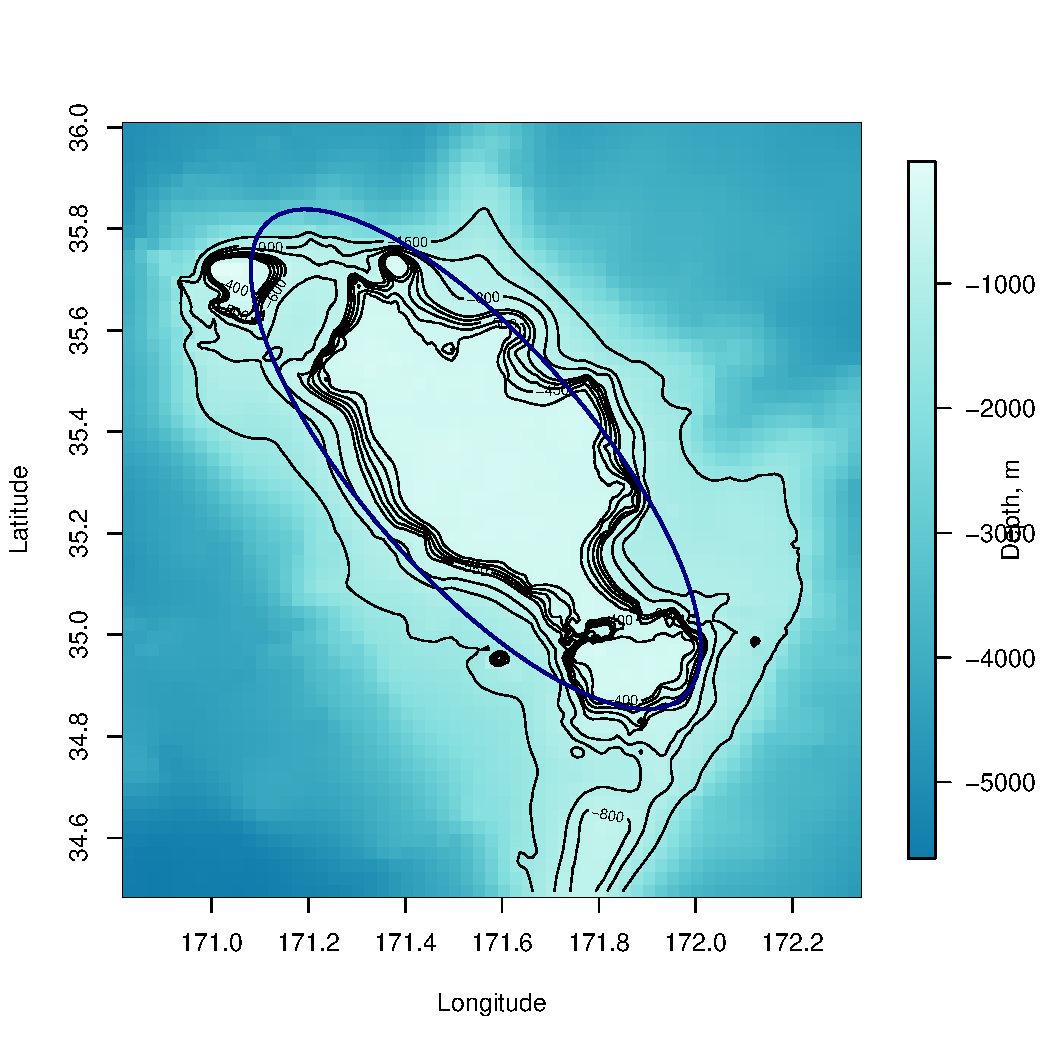
\includegraphics[scale=0.5]{../figures/koko_ell.pdf}
\end{figure}
Tsunami wave packet consists of many frequencies (fig. 2). Notable that most of the energy is associated with waves in range of minutes to one hour. For parametric study it should be chosen appropriate ranges for identifying principal physics. Following geometrical description based on simplified elliptical shape it is deduced 3 regimes (fig. 3):
\begin{itemize}
\item short period waves with wavelength less than major axis, $\lambda \leq 130 km$, $5 min < T < 12.5 min$
\item intermediate period waves with wavelength comparable $\lambda \sim 130 km$, $12.5 min < T < 20 min$
\item long period waves with wavelength larger $\lambda > 130 km$, $20 min < T$
\end{itemize}
For each regime is considered two periods which will be $T = 5, 10, 12.5, 17.5, 20, 22.5, 27.5, 30, 35$
\begin{figure}
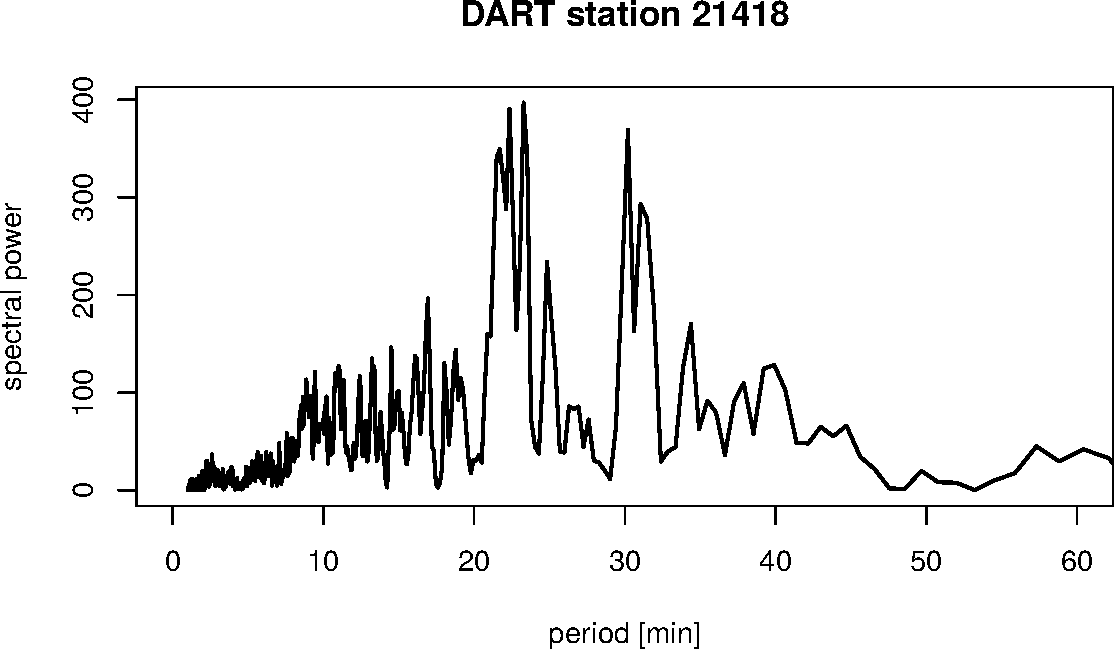
\includegraphics[scale=0.5]{../figures/tsunami_spectra.pdf}
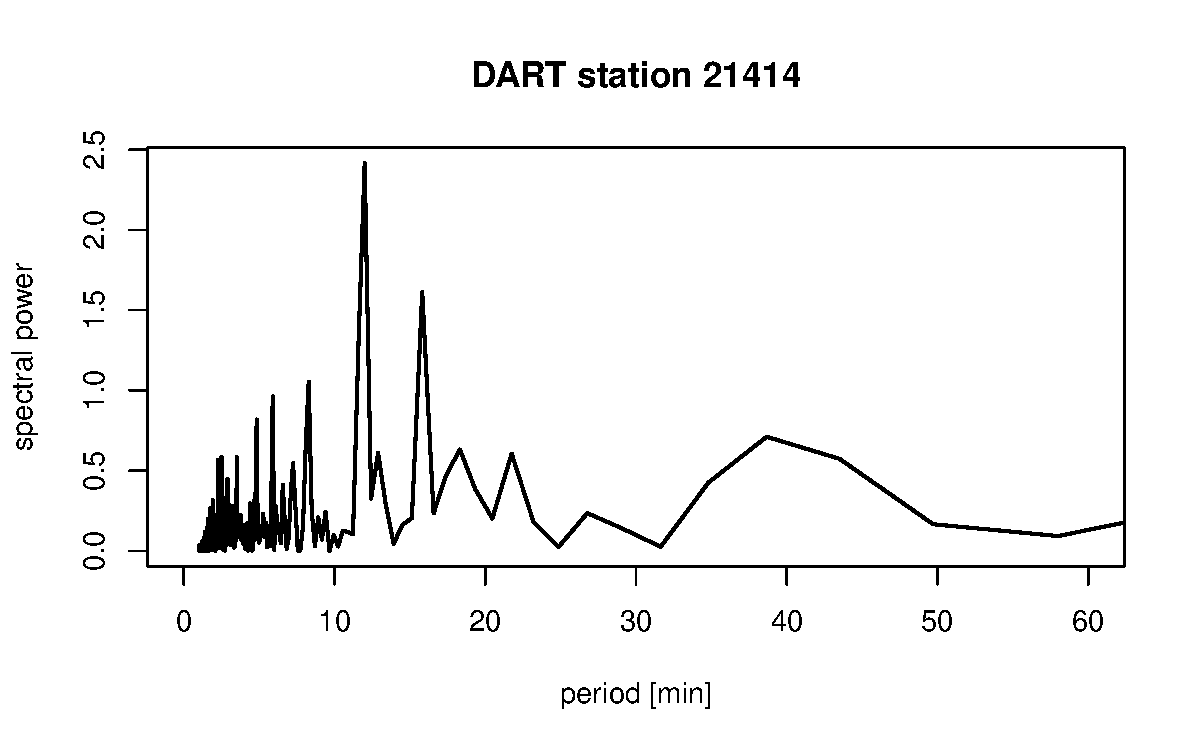
\includegraphics[scale=0.5]{../figures/spectra_tsunami_21414.pdf}
\caption{a) FFT of tsunami wave observed at DART station 21418 close to Japan after Tohoku event in 2011. b) Same for station 21414 after Kuril tsunami in November 2006.}
\end{figure}

\begin{figure}
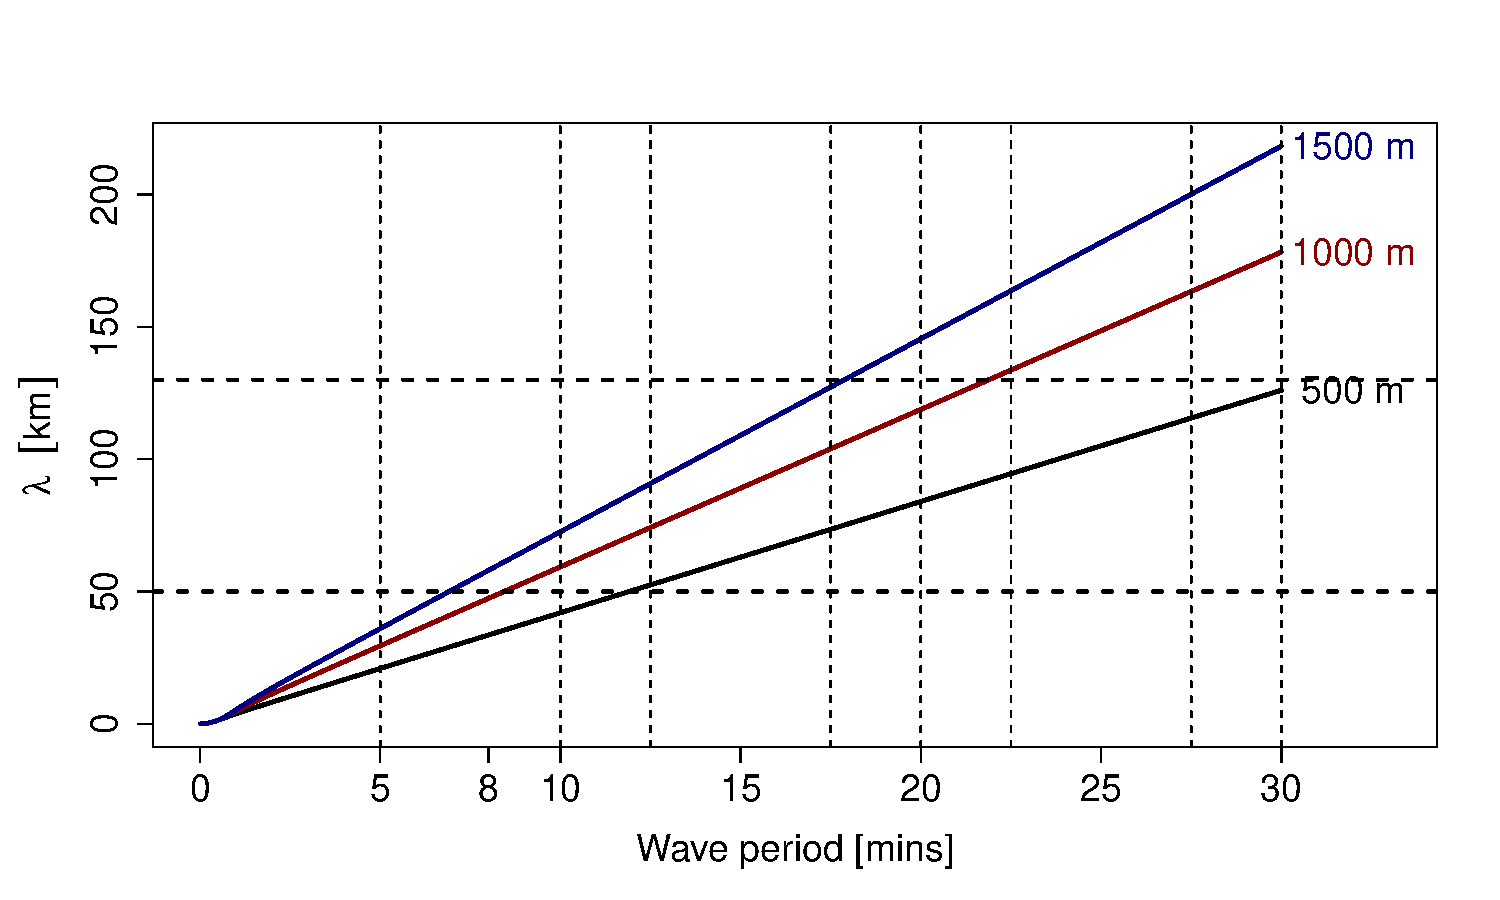
\includegraphics[scale=0.5]{../figures/tsunami_regimes.pdf}
\caption{Comparison of wavelength and seamountain sizes following dispersion relation for the surface gravity waves}
\end{figure}

In this investigation as well two tsunami events are kept in mind. The first tsunami was triggered by prominent earthquake in Japan, in March 2011. The second event happened due to Kuril earthquake in Novermber 2006. To investigate differences in wave-bathymetry interaction using ray tracing are found difference in wave incidence (Figure 3). It is clear the waves from the first event had more East-West direction while for Kuril event the waves approached Koko Guyot from Northwest.
\begin{figure}
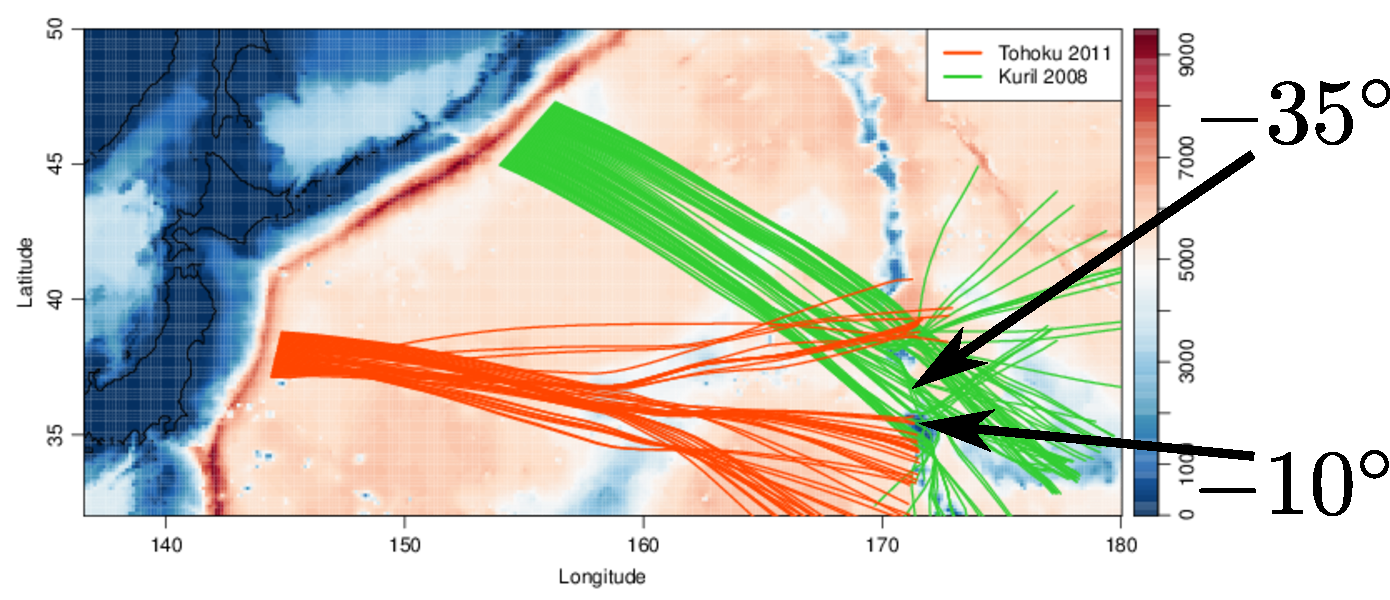
\includegraphics[scale=0.5]{../figures/koko_rays.pdf}
\caption{Comparison of wavelength and seamountain sizes following dispersion relation for the surface waves (all done on fingers, so REDO picture)}
\end{figure}

\newpage

\section{Numerical experiments of Kuril and Tohoku events}

\section{Analytical description of scattering by Koko Guoyt}

\section{Discussion}

\section{Conclusions}

\newpage
\section*{TO DO LIST}
\begin{itemize}
\item Angular decomposition and scattered wave field
\item Elliptic seamount, analytical solution
\item Windowing, wavelets of numerical results
\item Energetics in the two events
\end{itemize}

\bibliographystyle{apacite}
\bibliography{/home/dmitry/Bibtex_lib/}

\end{document}